Let $y$ be the position of a particle in one dimension, and let $t$ be time. So
there is just a single input variable: $t$.

An Ordinary Differential Equation is an equation relating the input variable
$t$ to $y$ and its derivatives. So, in general,
\begin{align*}
  f\(t, y, y', y'', \ldots\) = 0.
\end{align*}

A first-order ODE involves first derivatives only.

Consider the subset\footnote{I.e. $f(t, y, y') = 0$ can be rearranged to give
  $y'$ as a function of $t, y$.} of first-order ODEs that specify a velocity
$v(t, y)$ at each point in $(t, y)$ space. Thus this ODE contains all the
information needed to animate the motion of the particle, starting from any
point $(t_0, y_0)$. So the statement of the initial condition problem is
\begin{align*}
  \dydt = v(t, y) ~~~~~~~~~~ y(t_0) = y_0.
\end{align*}

The solution to an ODE is a function $y = \varphi(t)$ that describes a motion
of the particle having the specified velocities at each point it passes
through. I.e., if $y = \varphi(t)$ is a solution, then
\begin{align*}
  \frac{\d \varphi}{\dt} = v\Big(t, \varphi(t)\Big) ~~~~~~~~~~~~~\text{for all $t$}.
\end{align*}

We can think of $v$ as a surface over the $(t, y)$ plane. A solution is a curve
in the plane whose derivative is equal to the height of the surface $v$, at
every point on the curve.

The phase space of this problem is the set of all possible $(y, v)$ values.?


\section{Taxonomy}

\subsection{Linear DEs}
A \textbf{linear DE} can be written as $Ly = f$, where $L$
is a linear operator. The domain of $f$ is the same as the domain of
$y$.

Basically this means that derivatives of $y$ of any degree may appear, but they
may not be multiplied together. I.e.
\begin{align*}
  \sum_{n=0}^d P_i(t) \frac{\d^ny}{\dt^n}(t) = Q(t)
\end{align*}
is a linear DE of degree $d$. (The 0-th derivative is the function $y$ itself.)
The $P_i(t)$ and $Q(t)$ may be any (?) functions of the independent variable.

\textbf{Theorem}: Linear combinations of solutions of linear DEs are themselves
solutions.

If $Q(t) = 0$ then it is a \textbf{homogeneous linear DE}.

\subsection{First-order linear DEs: integrating factors}
A \textbf{first-order linear DE} can be written in the form
\begin{align*}
  y'(t) + P(t)y(t) = Q(t).
\end{align*}

First-order linear DEs can be solved by use of an \textbf{integrating factor}:
we seek $I(t)$ such that
\begin{align*}
  \Big(I(t)y(t)\Big)' = I(t)\Big(y'(t) + P(t)y(t)\Big),
\end{align*}
since then
\begin{align*}
  y(t) = \frac{1}{I(t)}\int I(t)Q(t) \dt + C.
\end{align*}

To find $I$, we want:
\begin{align*}
  \Big(I(t)y(t)\Big)' = I(t)\Big(y'(t) + P(t)y(t)\Big),
\end{align*}
i.e.
\begin{align*}
  I(t)y'(t) + I'(t)y(t) &= I(t)y'(t) + I(t)P(t)y(t)\\
  I'(t) &= I(t)P(t)\\
  \int \frac{1}{I(t)} \d I &= \int P(t) \dt\\
                        I &= Ae^{\int P(t) \dt},
\end{align*}
so we use $I(t) = e^{\int P(t) \dt}$.


\section{Special cases}
\subsection{Velocity depends on time only}
\begin{align*}
  \dydt = v(t)
\end{align*}
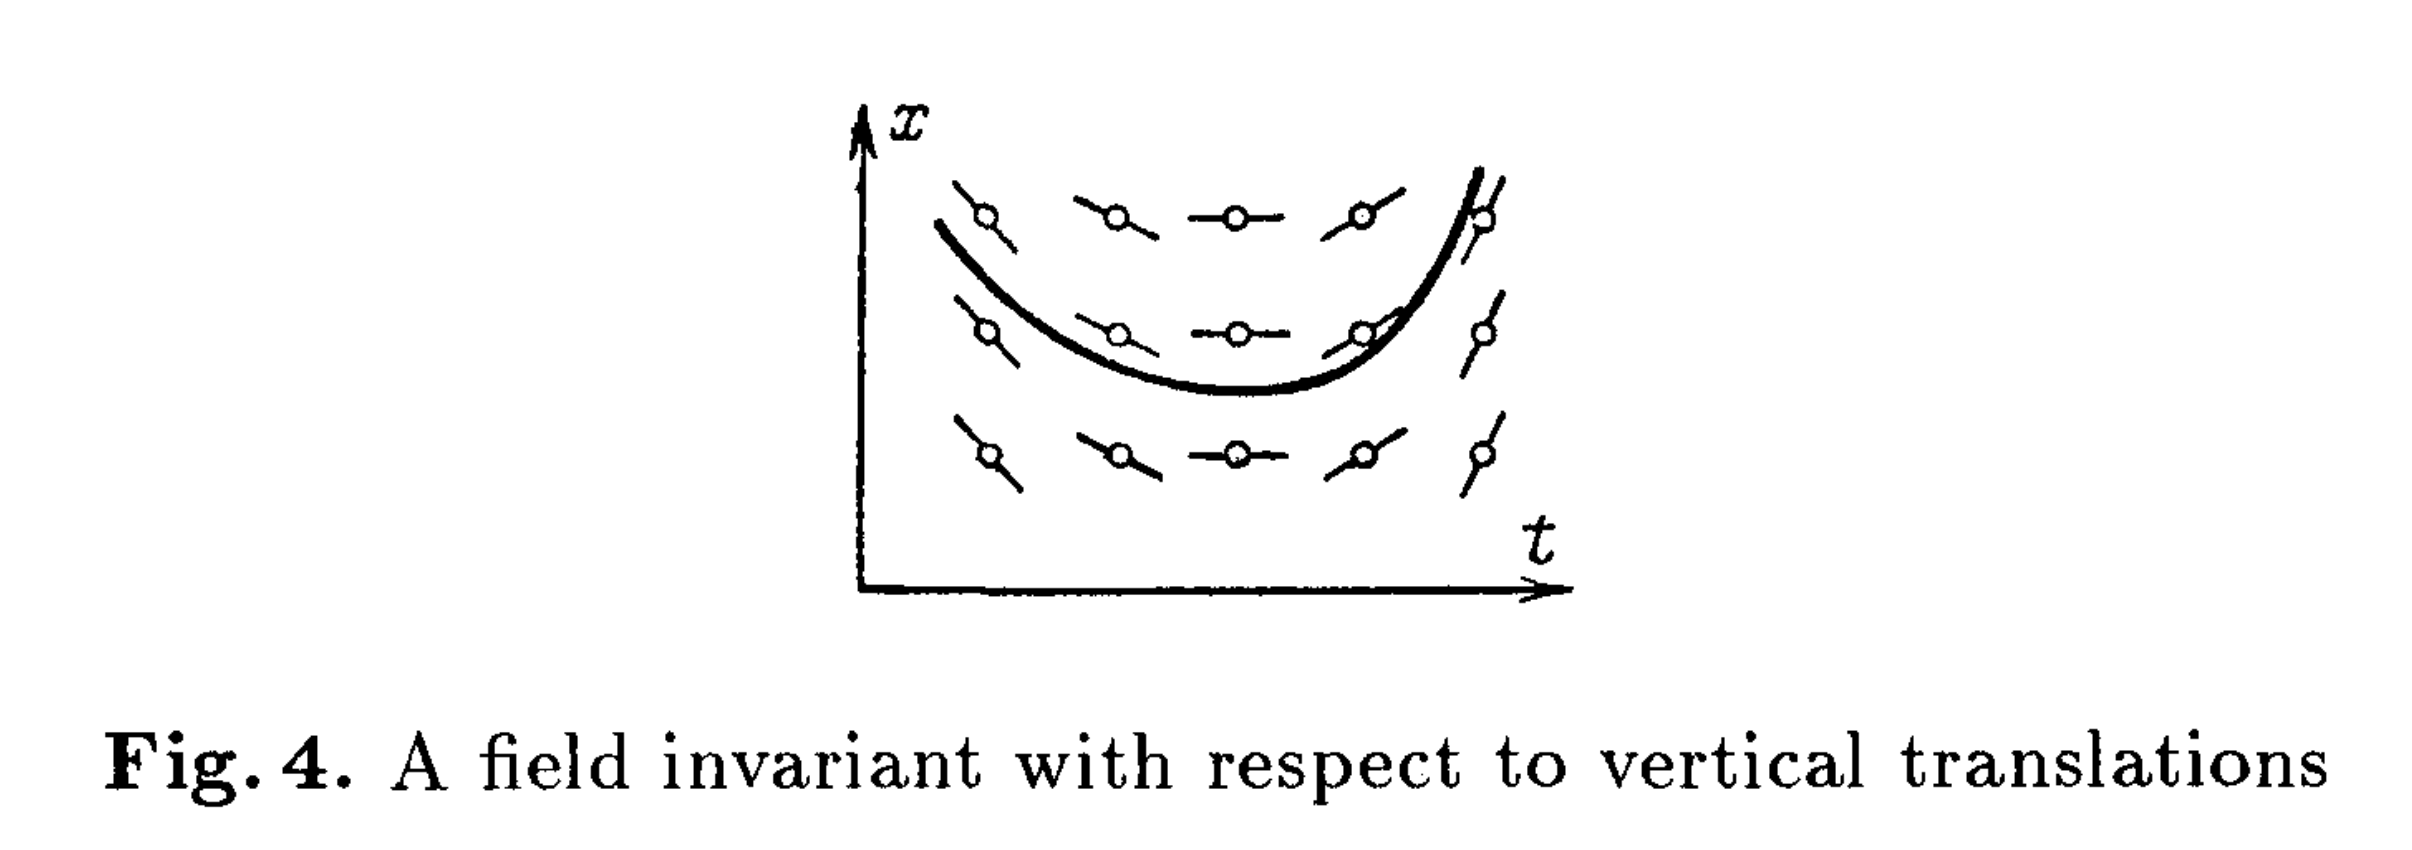
\includegraphics[width=340pt]{img/differential-equations-1-direction-field.png}\\
To find functions that solves this, one possibility is that we can find the
antiderivative explicitly:
\begin{align*}
  \int \dydt \dt := y(t) + C = \int v(t) \dt.
\end{align*}


\subsection{Velocity depends on location only (autonomous)}
\begin{align*}
  \dydt = v(y)
\end{align*}
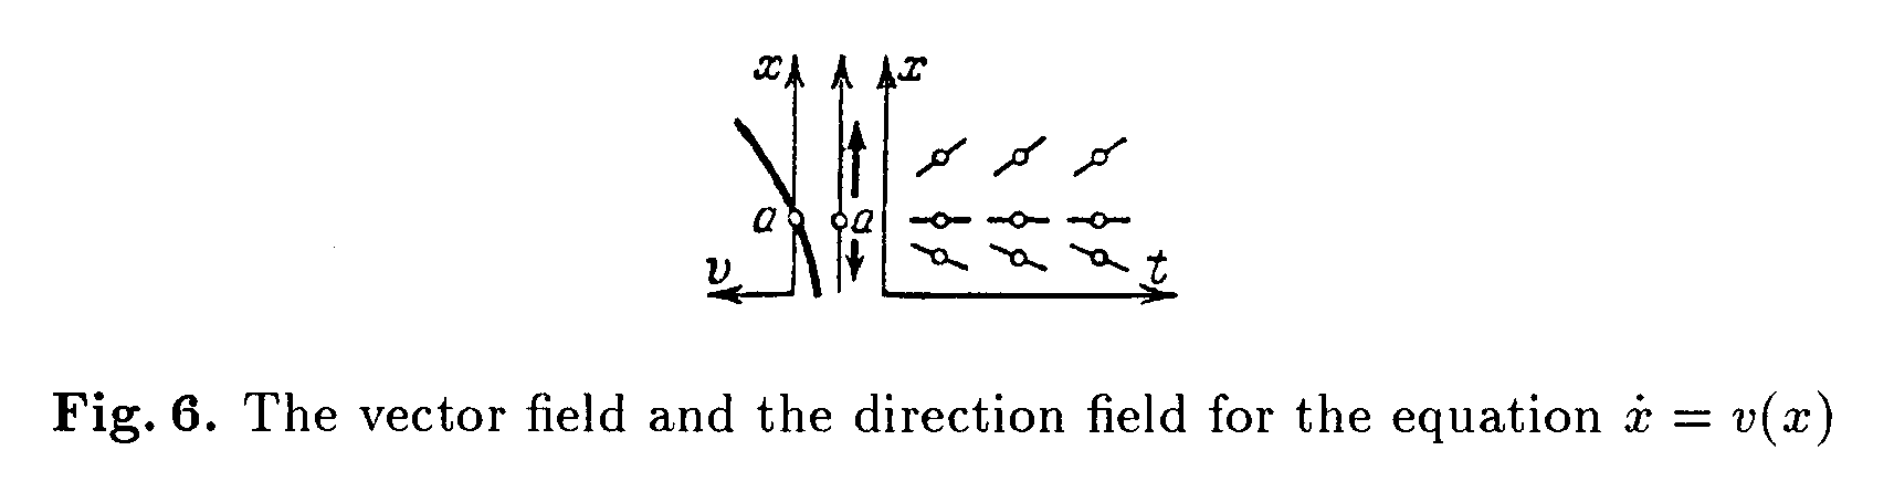
\includegraphics[width=400pt]{img/differential-equations-2-direction-field.png}\\



\section{Examples}
\subsection{C$^{14}$ dating}
\begin{mdframed}
  In a living organism the amount of C$^{14}$, as a proportion of all the
  C$^{12}$ and C$^{14}$, is expected to be a known constant $p_0$. After death,
  C$^{14}$ decays to C$^{12}$. How old is a specimen with proportion $p_1$ of
  C$^{14}$?
\end{mdframed}
Let $\lambda$ be the rate at which one atom of C$^{14}$ decays in atoms/sec. So
in a sample of $N$ atoms, the expected number to decay in one second is
$N\lambda$.

Let $N(t)$ be the number of C$^{14}$ atoms remaining at time $t$. We can
specify the model as a first-order ODE:
\begin{align*}
\frac{\d N}{\dt} = -N\lambda.
\end{align*}
Equivalently, dividing by the constant total number of carbon atoms,
\begin{align*}
\frac{\d p}{\dt} = -p\lambda,
\end{align*}
where $p(t)$ is the proportion of C$^{14}$ at time $t$.

It's easy to find a family of functions $p(t)$ that satisfies this differential equation. Since
\begin{align*}
  \frac{1}{p(t)} \frac{\d p}{\dt} = -\lambda,
\end{align*}
it must be the case that their antiderivatives are the same, up to a constant:
\begin{align*}
  \log(p(t)) &= -\lambda t + C\\
  p(t)  &= Ae^{-\lambda t}.
\end{align*}
Further, the expected proportion in a living organism determines a particular
function as the solution:
\begin{align*}
  p(0) = p_0 = Ae^{-\lambda . 0}
\end{align*}
so $A = p_0$ and the solution is
\begin{align*}
  p(t)  &= p_0e^{-\lambda t}.
\end{align*}
So the estimated age of a sample with proportion $p_1$ is
\begin{align*}
  t = \frac{1}{\lambda}\log\(\frac{p_0}{p_1}\).
\end{align*}



\section{Picard's Existence Theorem}
Consider again the initial value problem
\begin{align*}
  \dydt = v(t, y) ~~~~~~~~~~ y(t_0) = y_0.
\end{align*}


The ODE could also be written as
\begin{align*}
  y(t) = \int v\Big(t, y(t)\Big) \dt + C,
\end{align*}
but this is merely an equivalent restatement, since the definition of
indefinite integral is antiderivative. If we can find an antiderivative, then
fine. If not, note that by FTC, the following definite integral describes a
solution:
\begin{align*}
  y(t) = y(t_0) + \int_{t_0}^t v\Big(\tau, y(\tau)\Big) \d\tau.
\end{align*}
But this specifies $y(t)$ in terms of itself, since the velocity $v$ depends
not only on $t$ but also on the current position\footnote{for example, the rate
  of change of the proportion on carbon-14 depends on the current proportion of
  carbon-14.}.\\

\subsection{Definition: Lipschitz condition}
$v(t, y)$ is Lipschitz in the $y$ direction if there exists an upper bound $L$
on the absolute value of the straight line slope between any two points lying
on a vertical line. I.e. $\exists L > 0$ such that
\begin{align*}
  \Big|v(t, y_1) - v(t, y_0)\Big| \leq L\Big|y_1 - y_0\Big|
\end{align*}
for all pairs of points $(t, y_0)$, $v(t, y_1)$.

\subsection{Theorem: Picard's existence theorem}
\begin{mdframed}
Let $R$ be a rectangle of width $2h$ and height $2k$ and let
$(t_0, y_0)$ be the center of the rectangle. Suppose
\begin{enumerate}
\item Within $R$, $v(t, y)$ is continuous, with $|v(t, y)| \leq M$
\item $Mh \leq k$
\item Within $R$, $v(t, y)$ is Lipschitz in the $y$ direction, with bound $L$
  on the absolute value of the straight line slope between any two points.
\end{enumerate}

Then the initial value problem
\begin{align*}
  \dydt = v(t, y) ~~~~~~~ y(t_0) = y_0
\end{align*}
has a unique solution in $R$.
\end{mdframed}

\subsection{Examples}

In these cases, $|y'|$ and $\partiald{v}{y}$ are bounded in any rectangle.

\subsubsection{A}
$y' = v(x, y) = x^2 + y^2 ~~~~~~~ y(0) = 0$

So it can be approximated by Picard iterates. Is an explicit solution possible here?

\subsubsection{B}
$y' = (1 - 2x)y ~~~~~~~ y(0) = 1$

This can be solved explicitly by separation-of-variables:
\begin{align*}
  \log(y) &= x- x^2 + C\\
  y       &= Ae^{x(1-x)}.
\end{align*}


\subsection{Non-examples}

$|y'|$ is bounded in any rectangle for all these examples. However,
$\partiald{v}{y}$ is not. Picard's theorem guarantees unique solutions only in
rectangles excluding such problematic points.

\subsubsection{A}
$y' = v(x, y) = 3y^{2/3}  ~~~~~~~ y(0) = 0$

$\partiald{v}{y} = 2y^{-1/3} \to \pm \infty$ at $y=0$.


\subsubsection{B}
$y' = v(x, y) = x^2y^{1/5} ~~~~~~~ y(0) = b$

$\partiald{v}{y} = \frac{1}{5}x^2y^{-4/5}$ which is not defined at $y=0$.

\subsubsection{C}
$y' = v(x, y) = y^2       ~~~~~~~ y(0) = 1$

$\partiald{v}{y} = 2y$, so seems like it should be fine. Solve by
separation-of-variables:

\begin{align*}
  \int y^{-2} y' \dx &= x + C\\
  -y^{-1}            &= x + C\\
  y                 &= \frac{1}{C - x}.
\end{align*}
The solution passing through the initial value $y(0) = 1$ is
\begin{align*}
  y                  &= \frac{1}{1 - x},
\end{align*}
which does not exist for all $x$ in the rectangle.

\newpage

\subsection{Gronwall's inequality}

\begin{theorem*}[Gronwall's inequality]
  Let $t_0, y_0$ and $\lambda$ be known constants, and let $y$ be a non-negative
  continuous function. Suppose that
  \begin{align*}
    y(t) \leq y_0 + \lambda\Bigg|\int_{t_0}^t y(\tau) \d\tau\Bigg|.
  \end{align*}
  Then
  \begin{align*}
    y(t) \leq y_0e^{\lambda(t - t_0)}.
  \end{align*}
\end{theorem*}

\begin{mdframed}
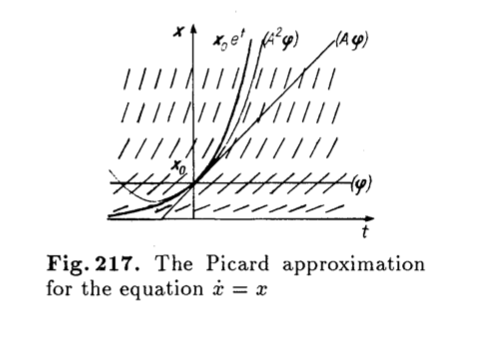
\includegraphics[width=200pt]{img/differential-equations-picard-gronwall.png}
\end{mdframed}

\begin{remark*}
  I think something close to the following is true: The above diagram from
  Arnold is strongly suggestive of Gronwall's inequality. If the Picard
  successive approximation procedure maps a function $\varphi$ onto itself,
  then that's a solution. The only other possibility is that it maps $\varphi$
  onto a function $A\varphi$ which is strictly greater. In that case, $\varphi$
  is bounded above by the true solution.
\end{remark*}

\begin{remark*}
  If we had equality instead of the inequality, then differentiation would give
  \begin{align*}
    y'(t) = \lambda y(t).
  \end{align*}
  This is the just the differential equation version of the integral equation
  with which we started. Recall that the general form of an ODE is
  \begin{align*}
    y'(t) = v(t, y(t)),
  \end{align*}
  so here we have $v(t, y(t)) = Ay(t)$. In other words, the direction field
  does not depend on $t$, as in Arnold's diagram.

  The solution to this ODE, with initial state $y(t_0) = y_0$, is
  \begin{align*}
    y(t) = y_0e^{\lambda(t - t_0)}.
  \end{align*}
  So Gronwell's inequality is saying that $y$ is bounded above by the solution
  to the differential equation that results from replacing the inequality with
  equality.
\end{remark*}

\begin{proof}

\end{proof}

\subsection{Contraction mapping theorem}
The following images are from Arnold, \textit{Ordinary Differential Equations}.\\

\begin{mdframed}
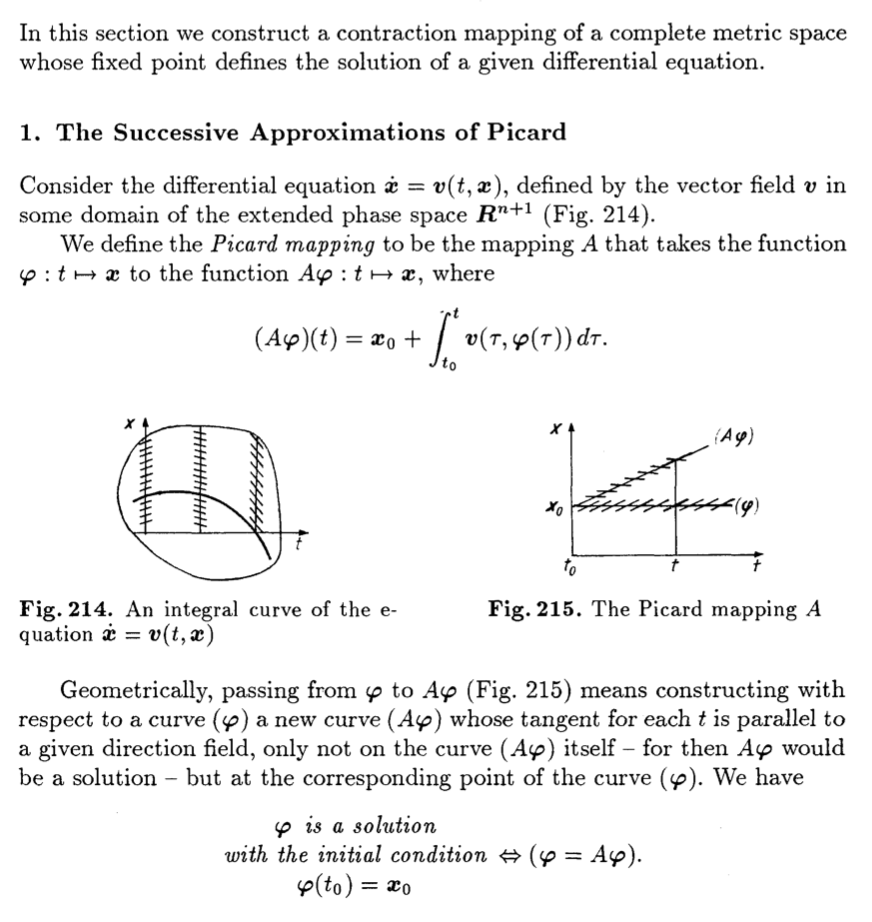
\includegraphics[width=400pt]{img/differential-equations-picard-contraction-mapping-fixed-point-arnold.png}
\end{mdframed}

\begin{mdframed}
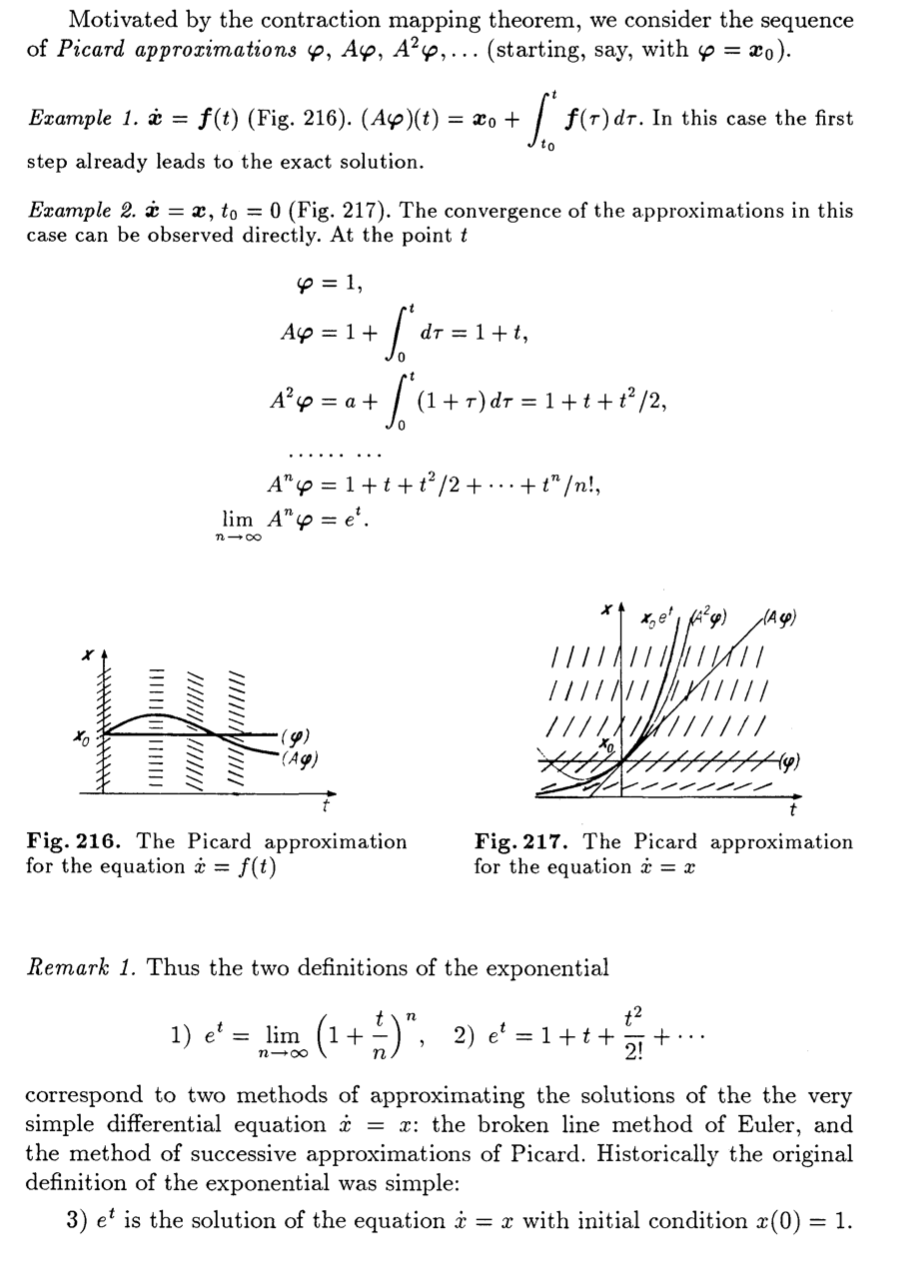
\includegraphics[width=400pt]{img/differential-equations-picard-contraction-mapping-fixed-point-arnold-2.png}
\end{mdframed}


\newpage
\subsection{Proof of Picard's existence theorem}

Consider the sequence of functions
\begin{align*}
  y_0(t) &= y_0\\
  y_n(t) &= y_0 + \int_{t_0}^t v\Big(\tau, y_{n-1}(\tau)\Big) \d\tau.\\
\end{align*}
We will show that
\begin{enumerate}
\item the $y_n(t)$ converge to a function $y_\infty(t)$;
\item $y_\infty(t)$ is a solution;
\item $y_\infty(t)$ is the only solution.
\end{enumerate}

\subsubsection{Proof that the $y_n(t)$ converge uniformly to a function $y_\infty(t)$}
The basic idea is to write the limiting function $y_\infty(t)$ as a telescoping
sum, and then to show that the series thus defined converges.

Define
\begin{align*}
  e_n(t) = y_{n+1}(t) - y_n(t), ~~~~~~~ n = 0, 1, 2, \ldots.
\end{align*}
Then the limiting function that is our objective is
\begin{align*}
  y_\infty(t) = y_0 + \sum_{n=0}^\infty e_n(t),
\end{align*}
if the series converges.

We are going to use the Weierstrass M-test to show that the series of functions
$\sum_{n=0}^\infty e_n(t)$ converge uniformly. So, we need to show that each
$e_n$ is bounded in absolute value by some constant $W_n$, and that the series
$\sum_{n=0}^\infty W_n$ converges.

For $n \geq 1$ each term is
\begin{align*}
  e_{n}(t) = \int_{t_0}^t v\Big(\tau, y_n(\tau)\Big) -
                         v\Big(\tau, y_{n-1}(\tau)\Big) \dt.
\end{align*}

Now, by assumption, $v$ is Lipschitz in the $y$ direction with bound
$L$. (Informally, this means that the absolute value of the straight line slope
between any two points lying on a vertical line is bounded by $L$). Therefore
\begin{align*}
      \Big|v\Big(t, y_n(t)\Big) -
           v\Big(t, y_{n-1}(t)\Big)\Big|
\leq L\Big|y_n(t) - y_{n-1}(t)\Big|.
\end{align*}
And since $\Big|\int_a^b f(t) \dt\Big| \leq \int_a^b |f(t)| \dt$,
\begin{align*}
  |e_n(t)|
  &\leq L\Bigg|\int_{t_0}^t \Big|y_n(\tau) - y_{n-1}(\tau)\Big| \d\tau \Bigg|\\
  &   = L\Bigg|\int_{t_0}^t \Big|e_{n-1}\Big| \d\tau \Bigg|.
\end{align*}
\footnote{The outer modulus is required to handle the case $t < t_0$.}

For the Weierstrass M-test we need to express the RHS as a constant $W_n$,
depending only on $L, M, n, t_0, y_0$. We will do this by induction.

For the first few terms we have
\begin{align*}
  |e_0(t)| &    = \Bigg|\int_{t_0}^t v(\tau, y_0) \d\tau\Bigg|\\
           & \leq M|t - t_0| ~~~~~~~~~~~~~~~~~~~~~~~~~~~~~~~~~~\text{(by assumption that $v$ is bounded by $M$)}\\
           & \leq Mh\\
  |e_1(t)| &    = L\Bigg|\int_{t_0}^t |e_0(\tau)| \d\tau\Bigg|  ~~~~~~~~~~~~~~~~~~~~~~~~\text{(by assumption that $v$ is Lipschitz in $y$)}\\
           & \leq L\Bigg|\int_{t_0}^t M|\tau - t_0| \d\tau\Bigg|\\
           &    = LM\frac{|\tau - t_0|^2}{2} \Big|_{t_0}^t \\
           &    = LM\frac{|t - t_0|^2}{2} \\
  |e_2(t)| &    = L\Bigg|\int_{t_0}^t |e_1(\tau)| \d\tau\Bigg|  ~~~~~~~~~~~~~~~~~~~~~~~~\text{(by assumption that $v$ is Lipschitz in $y$)}\\
           & \leq L\Bigg|\int_{t_0}^t LM\frac{|t - t_0|^2}{2} \d\tau\Bigg|\\
           &    = L^2M\frac{|t - t_0|^3}{3!}.
\end{align*}
So it seems that\\

\begin{lemma} \label{picard-convergence-induction}
Suppose
\begin{enumerate}
\item $|e_0(t)| \leq Mh$,
\item $|e_n(t)| \leq L\Bigg|\int_{t_0}^t \Big|e_{n-1}\Big| \d\tau \Bigg|$ for $n \geq 1$.
\end{enumerate}
Then
\begin{align*}
|e_n(t)| \leq L^nM\frac{h^{n+1}}{(n+1)!} =: W_n.
\end{align*}
Furthermore, $\lim_{n\to\infty}W_n = 0$.
\end{lemma}

\begin{proof}
To prove this, note that we know it is true of $e_0$. So suppose it is true of
$e_n$. Then the next term is
\begin{align*}
  |e_{n+1}(t)| & :=   \Big|y_{n+2}(t) - y_{n+1}(t)\Big|\\
              & \leq L\Bigg|\int_{t_0}^t \Big|y_{n+1}(\tau) - y_{n}(\tau)\Big| \d\tau\Bigg|\\
              &=     L\Bigg|\int_{t_0}^t |e_n(\tau)| \d\tau\Bigg|\\
              &=     L\Bigg|\int_{t_0}^t L^nM\frac{|\tau - t_0|^{n+1}}{(n+1)!} \d\tau\Bigg|\\
              &=     L^{n+1}M\frac{|t - t_0|^{n+2}}{(n+2)!^{~~~}}\\
              & \leq L^{n+1}M\frac{h^{n+2}}{(n+2)!^{~~~}},
\end{align*}
so
\begin{align*}
|e_n(t)| \leq L^nM\frac{h^{n+1}}{(n+1)!}
\end{align*}
for all $n \geq 0$ by induction.

According to the Ratio Test for convergence of a series, we examine
\begin{align*}
  \lim_{n\to \infty} \frac{W_{n+1}}{W_n}
  &= \lim_{n\to\infty} \frac{L^{n+1}M\frac{h^{n+2}}{(n+2)!}}
                          {L^nM\frac{h^{n+1}}{(n+1)!}}
   = \lim_{n\to\infty} \frac{Lh}{n+2}
    = 0,
\end{align*}
proving that the series $\sum_{n=0}^\infty W_n$ converges.
\end{proof}

To summarize:
\begin{enumerate}
\item Each $e_n(t)$ is bounded in absolute value by $W_n = L^nM\frac{h^{n+1}}{(n+1)!}$
\item The series $\sum_{n=0}^\infty W_n$ converges, by the Ratio Test.
\item Therefore the series $\sum_{n=0}^\infty e_n(t)$ converges uniformly, by
  the Weierstrass M-test.
\item Therefore the sequence $(y_n)_{n\geq 0}$ converges uniformly to a
  limiting function $y_\infty(t)$, since
  $\sum_{n=0}^\infty e_n(t) = y_\infty(t) - y_0$.
\end{enumerate}

\subsubsection{Proof that $y_\infty(t)$ is a solution}

To prove that the limiting function $y_\infty$ is a solution, we need to show
that
\begin{align*}
  y'_\infty(t) = v(t, y_\infty(t)) \text{~~~~~~~and~~~~~~~} y_\infty(t_0) = y_0.
\end{align*}

Recall the definition of the Picard successive approximations:
\begin{align*}
    y_n(t) &= y_0 + \int_{t_0}^t v\Big(\tau, y_{n-1}(\tau)\Big) \d\tau.
\end{align*}
Certainly, $y_\infty(t_0) = y_0$. And
\begin{align*}
  y_\infty(t) = \lim_{n\to \infty} y_n = y_0 + \int_{t_0}^t v(\tau, y_\infty(\tau)) \d\tau
\end{align*}
as long as it is justified to take the limit inside the integral.

This would be justified if $v(\tau, y_n(\tau))$ converges uniformly to
$v(\tau, y_\infty(\tau))$. These are two different functions, both mapping $t$
to the first derivative. Let's write them as $v_{y_n}(t)$ and
$v_{y_\infty}(t)$. We're looking for uniform convergence of the former to the
latter, i.e. uniform over all values of $t$. The definition of uniform
convergence is that there exists real $\epsilon > 0$ and integer $N \geq 0$
such that for all $t$, if $n > N$ then
$|v_{y_\infty}(t) - v_{y_n}(t)| < \epsilon$.

By assumption $v$ is Lipschitz in the $y$ direction, so
\begin{align*}
  |v(t, y_1) - v(t, y_2)| \leq L|y_1 - y_2| \leq 2Lk ~~~~~~~\forall y_1, y_2 \in [-k, k],
\end{align*}
giving the bound needed to prove uniform convergence.

Therefore
\begin{align*}
  y_\infty(t) = y_0 + \int_{t_0}^t v(\tau, y_\infty(\tau)) \d\tau,
\end{align*}
and therefore, by differentiating both sides,
\begin{align*}
  y'_\infty(t) = v(t, y_\infty(t)).
\end{align*}

\subsubsection{Proof that $y_\infty(t)$ is the unique solution}

We've shown that $(y_n)_{n\geq 0}$ converges to a solution $y_\infty$. Now we
need to show that if $Y$ is a solution then $Y = y_\infty$.

Recall that the proof of convergence relied on the following:
\begin{enumerate}
\item The definition of $e_n$ meant that $e_n$ could be expressed in terms of $e_{n-1}$.
\item A bound for the first term $e_1$ was provided by the assumption that $v$
  was bounded. Informally, this placed a bound on the amount of $v$ height
  difference that could be accumulated by $y_1$ between $t_0$ and $t$.
\item A bound for subsequent terms could be expressed in terms of the bound for
  the previous term. Informally, this was because the subsequent terms involved
  differences in $v$ height, which are bounded due to the Lipschitz
  assumption.
\end{enumerate}

We now need to do something similar to demonstrate that if $Y$ is a solution,
then $y_n \to Y$ as $n \to \infty$.

So suppose $Y$ is a solution. Then
\begin{align*}
  Y(t) = y_0 + \int_{t_0}^t v(\tau, Y(\tau)) \d\tau.
\end{align*}
Define $d_n(t) = Y(t) - y_n(t)$. We need to show that $|d_n(t)| \to 0$ for all
$t$ as $n \to \infty$.\\

\begin{mdframed}
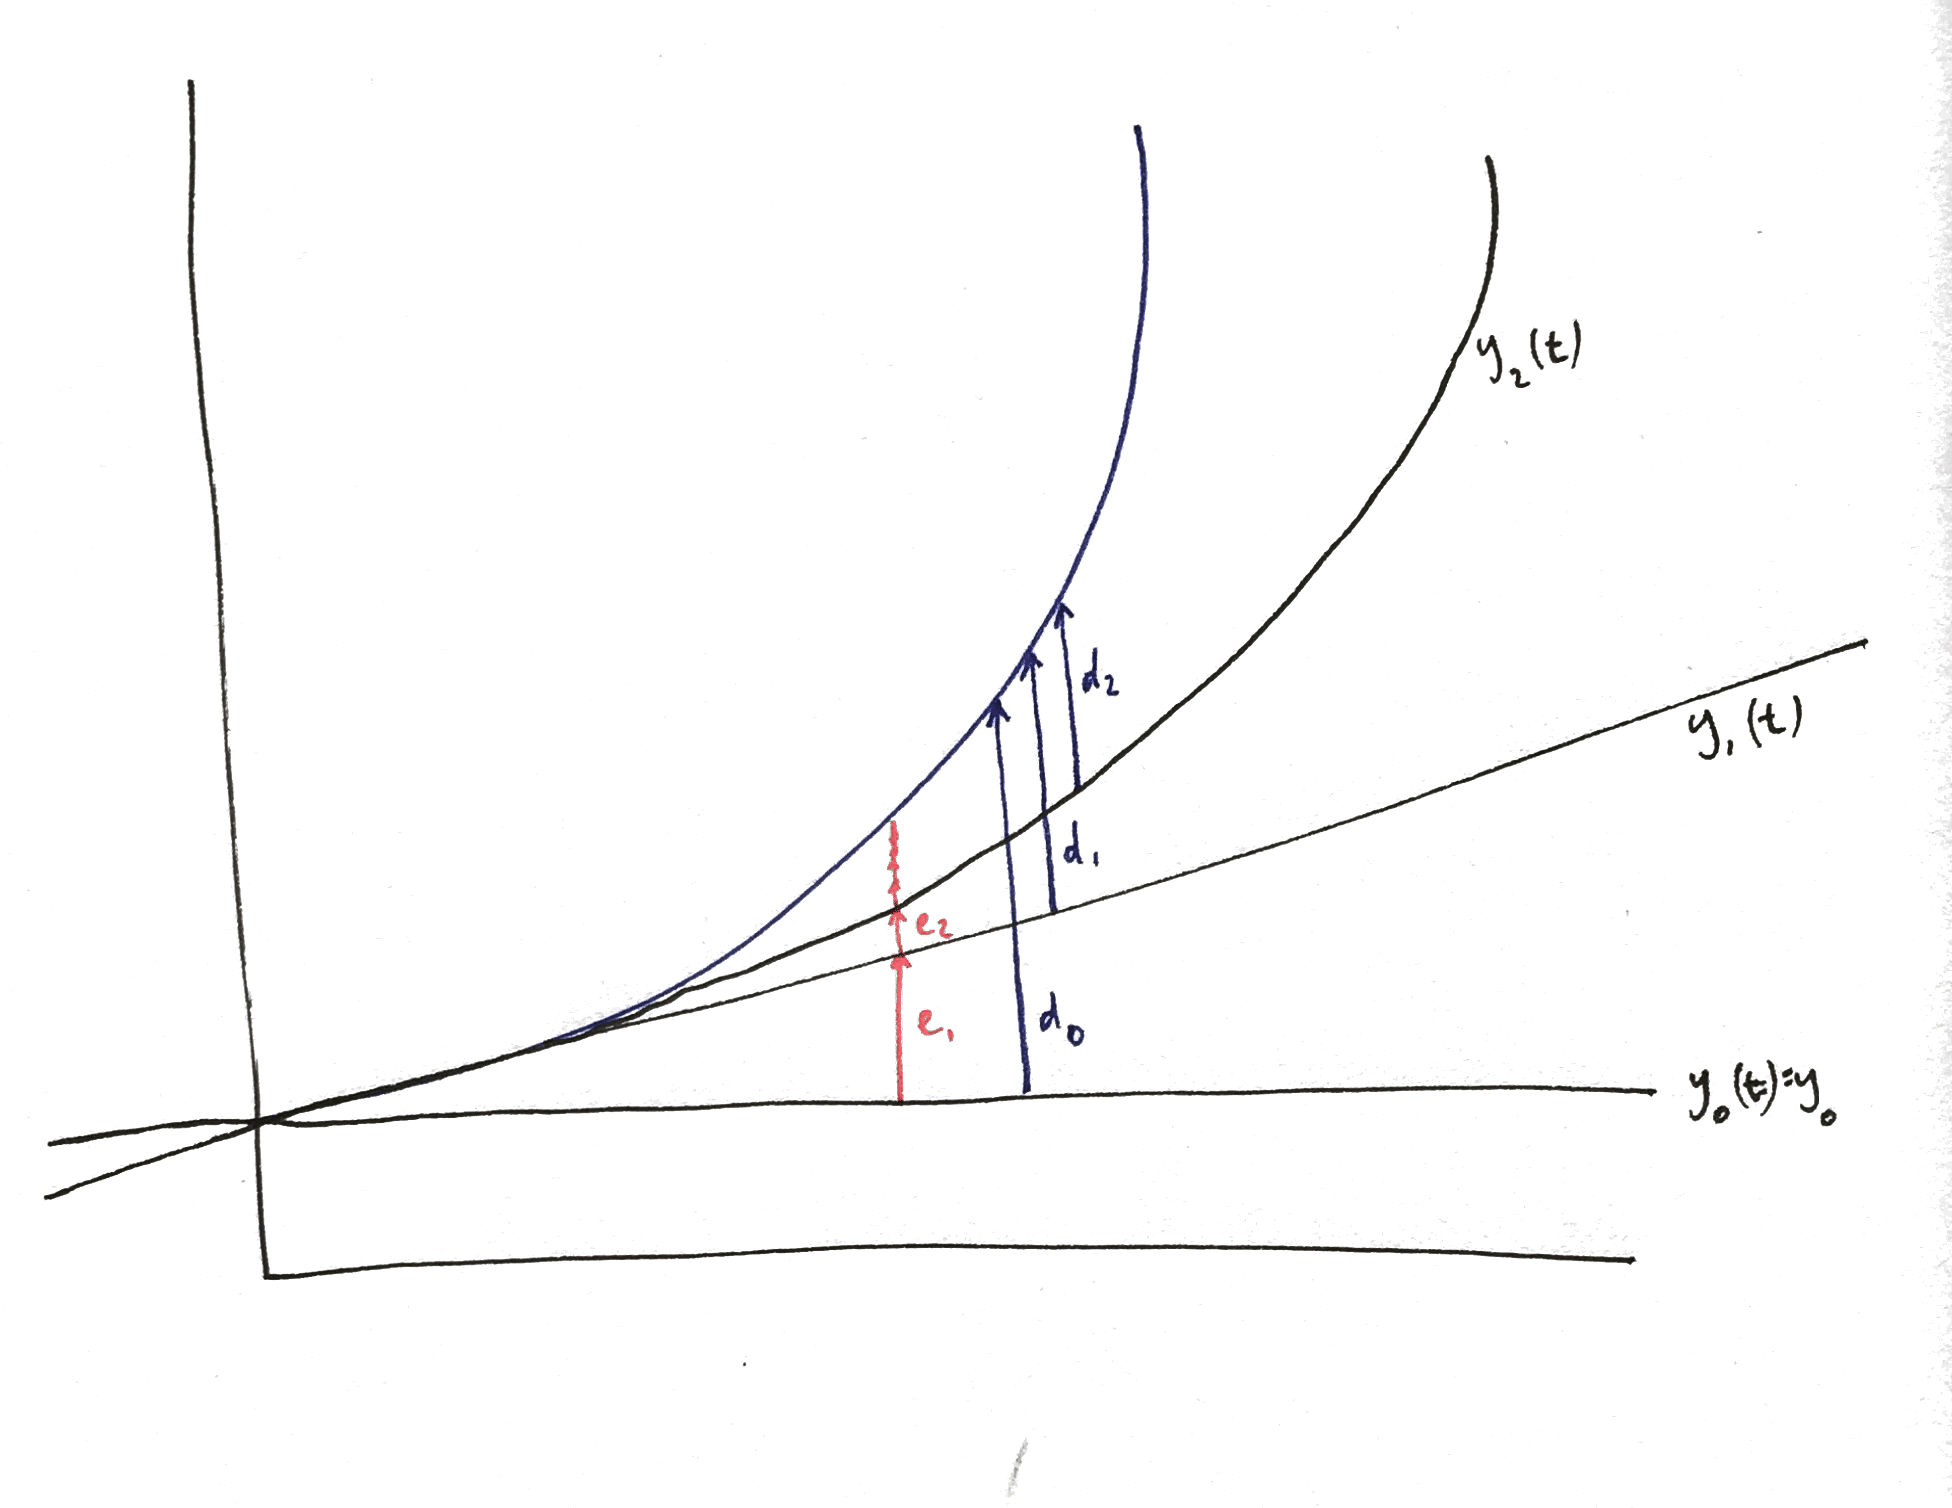
\includegraphics[width=250pt]{img/differential-equations-picard-convergence-uniqueness.png}
\end{mdframed}

The first term is
\begin{align*}
  d_0(t) = \int_{t_0}^t v(\tau, Y(\tau)) \d\tau.
\end{align*}

As in the convergence proof, the fact that $v$ is assumed to be bounded
provides a bound:
\begin{align*}
  |d_0(t)| \leq M|t - t_0|.
\end{align*}
Subsequent terms are
\begin{align*}
  |d_n(t)| &=    \Big|Y(t) - y_n(t)\Big|\\
           &=    \Bigg|\int_{t_0}^t v(\tau, Y(\tau)) - v(\tau, y_{n-1}(\tau)) \d\tau\Bigg|\\
           &\leq \Bigg|\int_{t_0}^t \Big|v(\tau, Y(\tau)) - v(\tau, y_{n-1}(\tau))\Big| \d\tau\Bigg|.
\end{align*}
As in the convergence proof, this involves a difference in $v$ height, so we
can use the Lipschitz assumption to express $d_n$ in terms of $d_{n-1}$:
\begin{align*}
  |d_n(t)| &\leq \Bigg|\int_{t_0}^t L\Big|Y(\tau) - y_{n-1}(\tau)\Big| \d\tau\Bigg|\\
           &   = \Bigg|L\int_{t_0}^t \Big|d_{n-1}(\tau)\Big| \d\tau\Bigg|.
\end{align*}

Therefore we can apply Lemma \ref{picard-convergence-induction} with $d_n(t)$
substituted for $e_n(t)$, to conclude that $d_n(t) \to 0$ as $n \to \infty$ for
all $t$, proving that if $Y$ is a solution, then $y_\infty = Y$. This completes
the proof of Picard's existence theorem. \qed


\newpage
\section{Simmons}

\subsection{Picard's theorem}
For every point $(t, y)$ in a rectangle, the ODE
\begin{align*}
  \dydt = f(t, y)
\end{align*}
has a solution passing through that point if $\partiald{f}{y}$ is Lipschitz
continuous in that rectangle.

\subsection{Families of curves}
For a family of curves, say the family of circles
\begin{align}
  x^2 + y^2 = c^2 \label{simmons-circles}
\end{align}
we can obtain a differential equation by implicit differentiation:
\begin{align}
  2x + 2y\dydx = 0. \label{simmons-circles-de}
\end{align}
Alternatively (eoc),
\begin{align*}
  (x + \dx)^2 + (y + \dy)^2 &= c^2\\
  x^2 + 2x\dx + y^2 + 2y\dy &= c^2\\
        2x\dx  + 2y\dy     &= 0.
\end{align*}

\subsection{Orthogonal trajectories}
What's the family of curves each of which is equal to every circle in \eqref{simmons-circles}?

Well, we know that their gradients are negative the inverse of the circle
gradients. So if we let $\dydx$ now be the gradient of the orthogonal
trajectories, then from \eqref{simmons-circles-de},
\begin{align*}
  2x - 2y\dxdy = 0
\end{align*}
is an ODE specifying the family of orthogonal trajectories. Thus
\begin{align*}
  \dydx &= \frac{y}{x}\\
  \log(y) &= \log(x) + C\\
       y &= Ax,
\end{align*}
so the orthogonal trajectories are lines through the origin, as expected.

\subsection{Use of polar coordinates to make a problem tractable (separable)}
TODO

\section{Arnold - Problems}
\subsection{}
\begin{mdframed}
  At what altitude is the density of the air one half of that at the surface of
  the Earth? Regard temperature as constant. One cubic meter of air at the
  Earth's surface weighs 1250g.
\end{mdframed}
\begin{align*}
  \rho(0) = 1250\\
  &=
\end{align*}